\documentclass{article}
\usepackage{tikz}
\usetikzlibrary{trees}

\begin{document}

    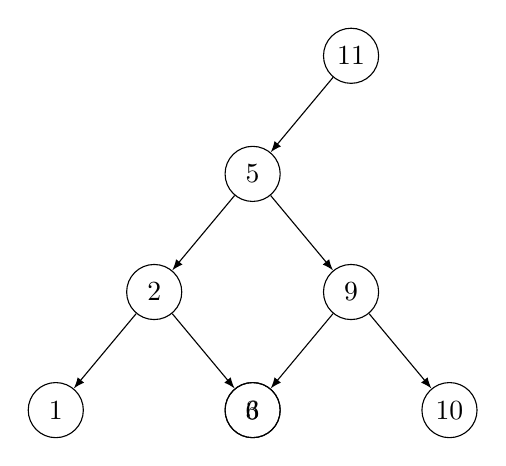
\begin{tikzpicture}[
        grow=down,
        level distance=1.5cm,
        sibling distance=2.5cm,
        every node/.style={circle, draw, minimum size=7mm, inner sep=2pt},
        edge from parent/.style={draw, -latex}
    ]
 \node {11}
     child {  node {5}
     child {  node {2}
     child {  node {1} }
     child {  node {3} } }
     child {  node {9}
     child {  node {6} }
     child {  node {10} } } }
     child [missing];
    \end{tikzpicture}

\end{document}
